\documentclass[tikz,border=6pt]{standalone}
\usepackage[T1]{fontenc}
\usepackage{helvet}\renewcommand{\familydefault}{\sfdefault}
\usepackage{amsmath,amssymb}
\usetikzlibrary{arrows.meta,positioning,calc,fit,backgrounds}
\definecolor{navy}{HTML}{16293D}\definecolor{teal}{HTML}{0E7C66}\definecolor{brick}{HTML}{C0392B}
\definecolor{amber}{HTML}{E8A33D}\definecolor{gold}{HTML}{A8801F}\definecolor{bodygrey}{HTML}{5A6672}
\begin{document}
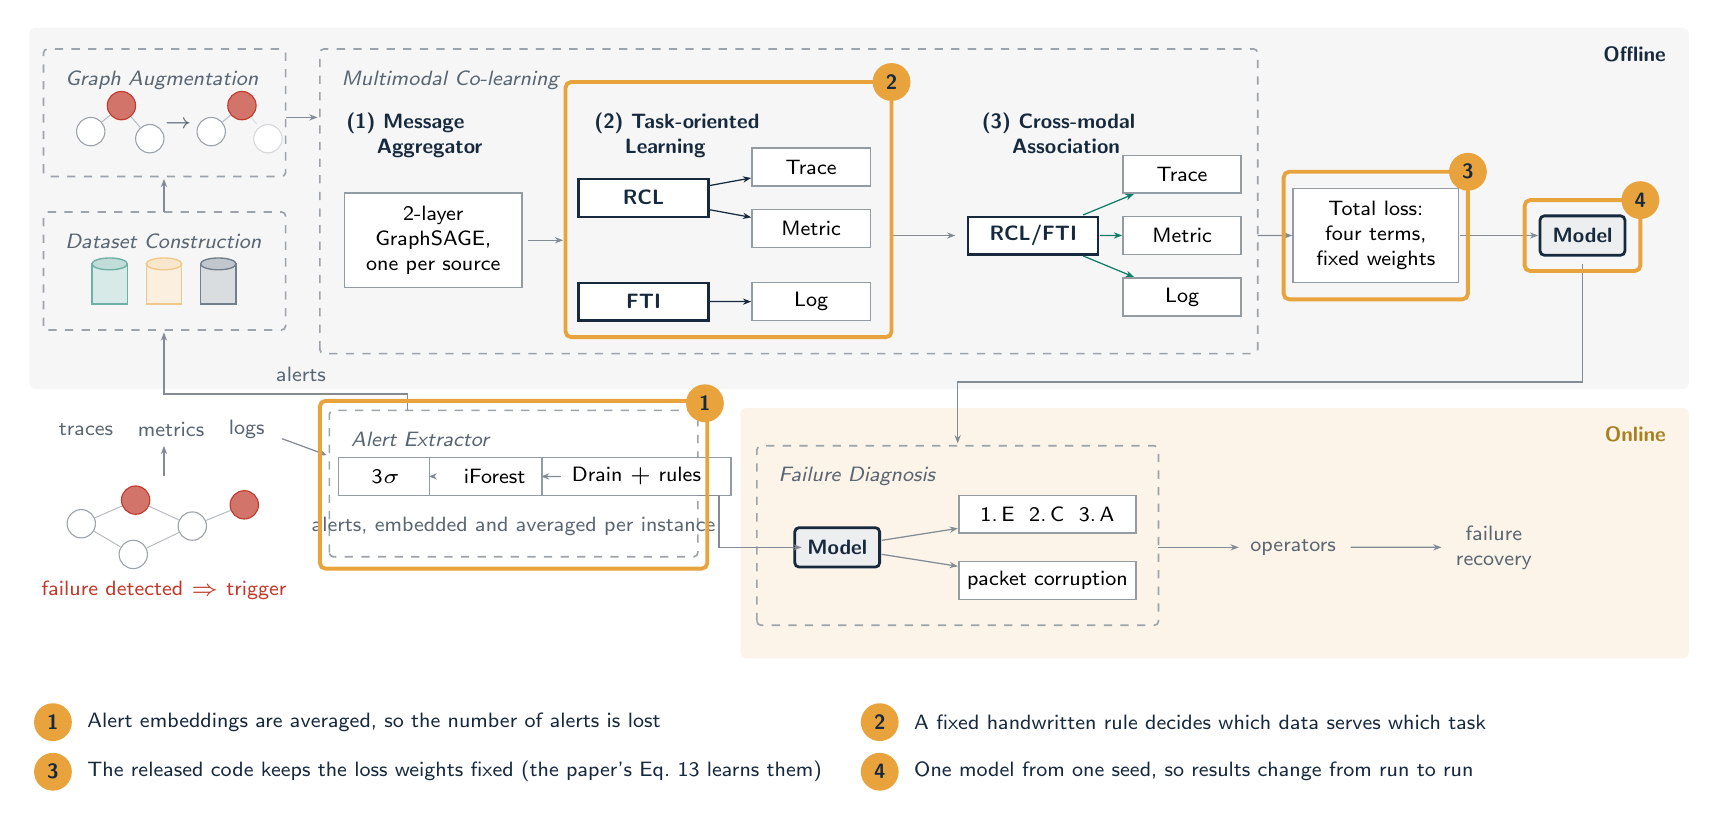
\begin{tikzpicture}[scale=1.5,every node/.style={transform shape},font=\scriptsize,
  mod/.style={draw=bodygrey!60,dashed,line width=0.6pt,rounded corners=1.5pt},
  ttl/.style={font=\tiny\itshape,color=bodygrey,anchor=north west},
  num/.style={font=\tiny\bfseries,color=navy,anchor=north west},
  bx/.style={draw=bodygrey!65,fill=white,line width=0.5pt,inner sep=1.7pt,font=\tiny,minimum width=10mm,minimum height=3.2mm},
  tk/.style={draw=navy,fill=white,line width=0.8pt,inner sep=1.7pt,font=\tiny\bfseries,text=navy,minimum width=11mm,minimum height=3.2mm},
  mdl/.style={draw=navy,fill=navy!8,line width=1.0pt,rounded corners=1.5pt,inner sep=3pt,font=\tiny\bfseries,text=navy},
  n/.style={circle,draw=bodygrey!60,fill=white,inner sep=0.7pt,minimum size=2.4mm},
  ar/.style={-{Stealth[length=3pt]},bodygrey!75,line width=0.45pt},
  new/.style={draw=amber,fill=amber!14,line width=0.8pt,rounded corners=1.2pt,inner sep=2pt,font=\tiny,text=navy,align=center},
  tag/.style={circle,fill=amber,text=navy,font=\tiny\bfseries,inner sep=0.9pt,minimum size=3.2mm},
  hl/.style={draw=amber,line width=1.4pt,rounded corners=2pt}]
\begin{scope}[opacity=1,text opacity=1]
\fill[navy!4,rounded corners=2pt] (-0.10,2.40) rectangle (13.95,5.46);
\node[anchor=north east,font=\tiny\itshape\bfseries,color=navy] at (13.88,5.42) {Offline};
\draw[mod] (0.02,4.20) rectangle (2.07,5.28);
\node[ttl] at (0.08,5.22) {Graph Augmentation};
\node[n] (g1) at (0.42,4.58) {}; \node[n,fill=brick!70,draw=brick] (g2) at (0.68,4.80) {};
\node[n] (g3) at (0.92,4.52) {};
\draw[bodygrey!45,line width=0.35pt] (g1)--(g2); \draw[bodygrey!45,line width=0.35pt] (g2)--(g3);
\node[font=\tiny,color=bodygrey] at (1.16,4.64) {$\to$};
\node[n] (h1) at (1.44,4.58) {}; \node[n,fill=brick!70,draw=brick] (h2) at (1.70,4.80) {};
\node[n,draw=bodygrey!25] (h3) at (1.92,4.52) {};
\draw[bodygrey!45,line width=0.35pt] (h1)--(h2);
\draw[bodygrey!22,dashed,line width=0.35pt] (h2)--(h3);
\draw[mod] (0.02,2.90) rectangle (2.07,3.90);
\node[ttl] at (0.08,3.84) {Dataset Construction};
\foreach \x/\c in {0.58/teal, 1.04/amber, 1.50/navy}{
  \draw[\c!60,fill=\c!16,line width=0.5pt] (\x-0.15,3.12) rectangle (\x+0.15,3.46);
  \draw[\c!60,fill=\c!26,line width=0.5pt] (\x,3.46) ellipse (0.15 and 0.05);}
\draw[ar] (1.04,3.90) -- (1.04,4.18);
\draw[mod] (2.36,2.70) rectangle (10.30,5.28);
\node[ttl] at (2.42,5.22) {Multimodal Co-learning};
\draw[ar] (2.07,4.70) -- (2.34,4.70);
\node[num] at (2.46,4.86) {(1) Message};
\node[num] at (2.46,4.64) {\ \ \ \ Aggregator};
\node[bx,minimum width=15mm,align=center,minimum height=8mm] (ma) at (3.32,3.66) {2-layer\\GraphSAGE,\\one per source};
\draw[ar] (4.12,3.66) -- (4.42,3.66);
\node[num] at (7.84,4.86) {(3) Cross-modal};
\node[num] at (7.84,4.64) {\ \ \ \ Association};
\node[tk] (rf) at (8.40,3.70) {RCL/FTI};
\node[bx] (tr2) at (9.66,4.22) {Trace};
\node[bx] (me2) at (9.66,3.70) {Metric};
\node[bx] (lo2) at (9.66,3.18) {Log};
\draw[ar,teal] (rf)--(tr2); \draw[ar,teal] (rf)--(me2); \draw[ar,teal] (rf)--(lo2);
\draw[ar] (7.20,3.70) -- (7.74,3.70);
\node[font=\tiny,color=bodygrey] at (0.38,2.06) {traces};
\node[font=\tiny,color=bodygrey] at (1.10,2.06) {metrics};
\node[font=\tiny,color=bodygrey] at (1.74,2.06) {logs};
\node[n] (s1) at (0.34,1.26) {}; \node[n,fill=brick!70,draw=brick] (s2) at (0.80,1.46) {};
\node[n] (s3) at (0.78,1.00) {}; \node[n] (s4) at (1.28,1.24) {};
\node[n,fill=brick!70,draw=brick] (s5) at (1.72,1.42) {};
\foreach \u/\v in {s1/s2,s1/s3,s2/s4,s3/s4,s4/s5}{\draw[bodygrey!45,line width=0.35pt] (\u)--(\v);}
\node[font=\tiny,color=brick,anchor=north] at (1.04,0.90) {failure detected $\Rightarrow$ trigger};
\draw[ar] (1.04,1.66) -- (1.04,1.92);
\draw[mod] (2.44,0.98) rectangle (5.56,2.22);
\node[ttl] at (2.50,2.16) {Alert Extractor};
\node[bx,minimum width=8mm] (ex1) at (2.92,1.66) {3$\sigma$};
\node[bx,minimum width=11mm] (ex2) at (3.84,1.66) {iForest};
\node[bx,minimum width=16mm] (ex3) at (5.04,1.66) {Drain $+$ rules};
\draw[ar] (ex1)--(ex2); \draw[ar] (ex2)--(ex3);
\node[font=\tiny,color=bodygrey,anchor=north] at (4.00,1.44) {alerts, embedded and averaged per instance};
\draw[ar] (2.04,1.98) -- (2.42,1.84);
\draw[ar,line width=0.55pt] (3.10,2.22) -- (3.10,2.36) -- (1.04,2.36) -- (1.04,2.88);
\end{scope}

\node[font=\tiny,color=bodygrey,anchor=south] at (2.20,2.34) {alerts};
% (2) task-oriented learning, fixed rule
\node[num] at (4.56,4.86) {(2) Task-oriented};
\node[num] at (4.56,4.64) {\ \ \ \ Learning};
\node[tk] (rcl) at (5.10,4.02) {RCL};
\node[tk] (fti) at (5.10,3.14) {FTI};
\node[bx] (tr) at (6.52,4.28) {Trace};
\node[bx] (me) at (6.52,3.76) {Metric};
\node[bx] (lo) at (6.52,3.14) {Log};
\draw[ar,navy] (rcl)--(tr); \draw[ar,navy] (rcl)--(me); \draw[ar,navy] (fti)--(lo);
% loss and model
\node[bx,minimum width=14mm,minimum height=8mm,align=center] (loss) at (11.30,3.70) {Total loss:\\four terms,\\fixed weights};
\draw[ar] (10.30,3.70) -- (loss.west);
\node[mdl] (model) at (13.05,3.70) {Model};
\draw[ar] (loss.east) -- (model.west);
% online
\fill[amber!12,rounded corners=2pt] (5.92,0.12) rectangle (13.95,2.24);
\node[anchor=north east,font=\tiny\itshape\bfseries,color=gold] at (13.88,2.20) {Online};
\draw[mod] (6.06,0.40) rectangle (9.46,1.92);
\node[ttl] at (6.12,1.86) {Failure Diagnosis};
\node[mdl] (m2b) at (6.74,1.06) {Model};
\node[bx,minimum width=15mm] (rk) at (8.52,1.34) {1.\,E\ \ 2.\,C\ \ 3.\,A};
\node[bx,minimum width=15mm] (ty) at (8.52,0.78) {packet corruption};
\draw[ar] (m2b)--(rk); \draw[ar] (m2b)--(ty);
\node[font=\tiny,color=bodygrey] (ops) at (10.60,1.06) {operators};
\node[font=\tiny,color=bodygrey,align=center] (rec) at (12.30,1.06) {failure\\recovery};
\draw[ar] (9.46,1.06) -- (10.14,1.06);
\draw[ar] (ops)--(rec);
\draw[ar,line width=0.55pt] (5.56,1.50) -- (5.74,1.50) -- (5.74,1.06) -- (6.44,1.06);
\draw[ar,line width=0.55pt] (13.05,3.46) -- (13.05,2.46) -- (7.76,2.46) -- (7.76,1.94);
% ---- highlighted areas under consideration
\draw[hl] (2.36,0.88) rectangle (5.64,2.30);   \node[tag] at (5.62,2.28) {1};
\draw[hl] (4.44,2.84) rectangle (7.20,5.00);   \node[tag] at (7.20,5.00) {2};
\draw[hl] (10.52,3.16) rectangle (12.08,4.24); \node[tag] at (12.08,4.24) {3};
\draw[hl] (12.56,3.40) rectangle (13.54,4.00); \node[tag] at (13.54,4.00) {4};
% ---- legend
\node[tag] (k1) at (0.10,-0.42) {1}; \node[anchor=west,font=\tiny,text=navy] at (k1.east) {Alert embeddings are averaged, so the number of alerts is lost};
\node[tag] (k2) at (7.10,-0.42) {2}; \node[anchor=west,font=\tiny,text=navy] at (k2.east) {A fixed handwritten rule decides which data serves which task};
\node[tag] (k3) at (0.10,-0.84) {3}; \node[anchor=west,font=\tiny,text=navy] at (k3.east) {The released code keeps the loss weights fixed (the paper's Eq.~13 learns them)};
\node[tag] (k4) at (7.10,-0.84) {4}; \node[anchor=west,font=\tiny,text=navy] at (k4.east) {One model from one seed, so results change from run to run};
\end{tikzpicture}
\end{document}
